\documentclass[a4paper, 12pt, french]{article}

\usepackage{babel}
\usepackage[T1]{fontenc}
\usepackage[utf8]{inputenc}
\usepackage{lmodern}

\usepackage{geometry}
\usepackage{graphicx}
\usepackage{tikz}

\newcommand*\circled[1]{
	\tikz[baseline=(char.base)]{
		\node[shape=circle,draw,inner sep=2pt] (char) {#1};
	}
}

% Define the margins
\geometry{top=2cm,left=2cm, right=2cm, bottom=2cm}

\title{Le jeu du taquin sous forme de système multi-agent}
\author{Guilhem \bsc{Marion} et Matthieu \bsc{Vieira}}
\date{juillet 2018}

\begin{document}

\maketitle

\section{Structure du programme}

Dans le cadre de l'UE Techniques de l'Intelligence Artificielle, nous avons construit un système multi-agents sur le modèle du jeu du taquin. Les agents sont dotés de capacités de raisonnement et de réactions indépendantes, ils sont capables de se déplacer sur la grille en même temps.

Notre programme, écrit en Python 3, est composé de deux fichiers :
\begin{itemize}
	\item \texttt{Puzzle.py} qui 
	\item \texttt{Agent.py}, une classe pour chaque agent qui est créé, chaque agent est un thread
\end{itemize}

[…]

Dans la suite de ce rapport, nous prendrons pour chaque exemple une grille de taille $n \times n$ avec $n = 5$, mais ce paramètre est évidemment modifiable.

\section{Construction des cas}

\subsection{Le cas à un agent}

\begin{figure}[h]
	\centering
	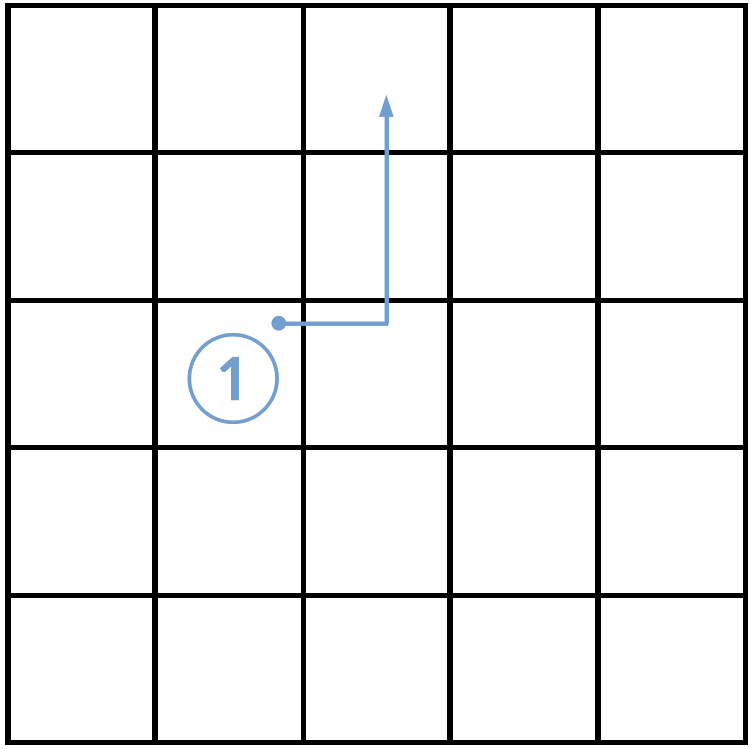
\includegraphics[width=200px]{images/base_case.png}
\end{figure}

C’est le cas le plus simple du programme. L'agent est seul sur la grille et a un objectif. Tant qu'il n'est pas sur sa case d'arrivée, l'agent calcule la distance par rapport à celle-ci pour chacune des cases sur laquelle il peut se déplacer. Dans le cas d'un quadrillage comme ici, la distance de Manhattan, donnée par la formule ci-dessous, est plus adaptée que la classique distance euclidienne.

\[
d(a, b) = |x_a - x_b| + |y_b - y_a|
\]

C'est le sens du code situé dans le fichier \texttt{Agent.py} des lignes 186 à 204 : le programme stocke dans une variable \texttt{dico} les 4 distances calculées, puis sélectionne la plus faible. Il se dirige alors sur la case correspondante et recommence un cycle avec un nouveau calcul des distances.

Dans le cas où deux directions sont possibles pour une distance de Manhattan, on choisit aléatoirement une des deux directions.

\begin{figure}[h]
	\centering
	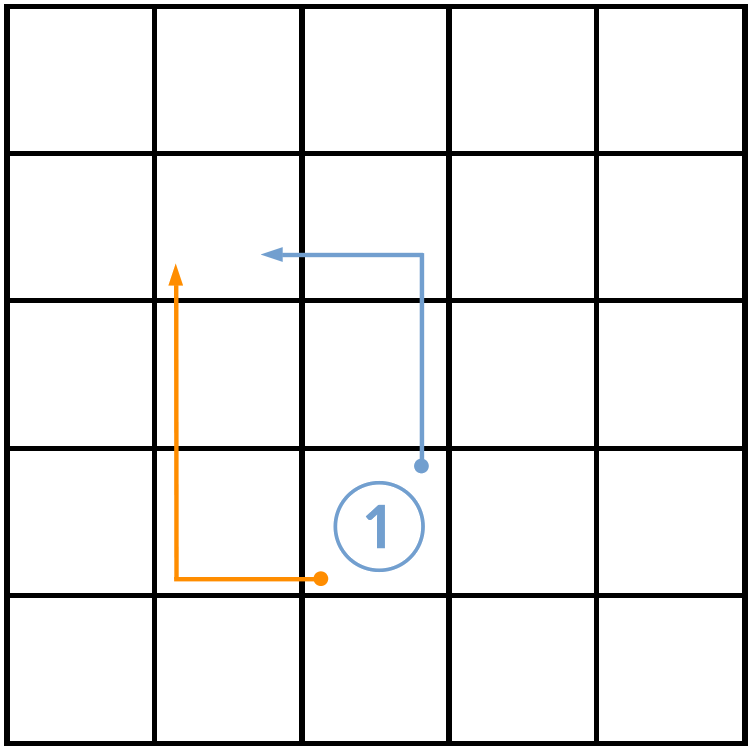
\includegraphics[width=200px]{images/manhattan_equal.png}
\end{figure}

Le cas à un agent ne présente aucun bloquage possible : l'agent arrive forcément sur sa case objectif, en empruntant le plus court chemin.

\subsection{Le cas à deux agents}

\begin{figure}[h]
	\centering
	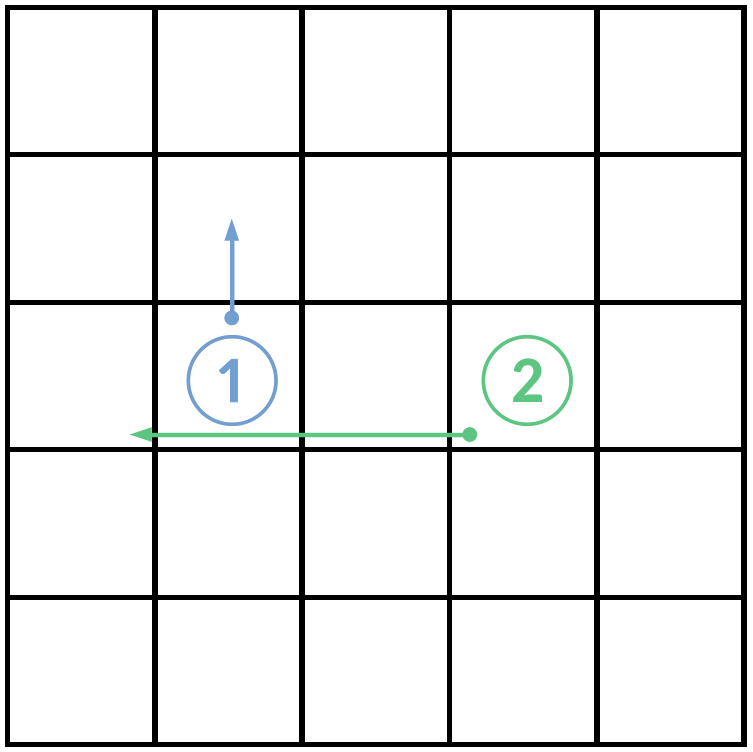
\includegraphics[width=200px]{images/2_agents.png}
\end{figure}

[…………… à compléter ………………]


Un premier cas pathologique peut apparaître dans cette configuration, comme le montre l'exemple ci-dessous.

\begin{figure}[h]
	\centering
	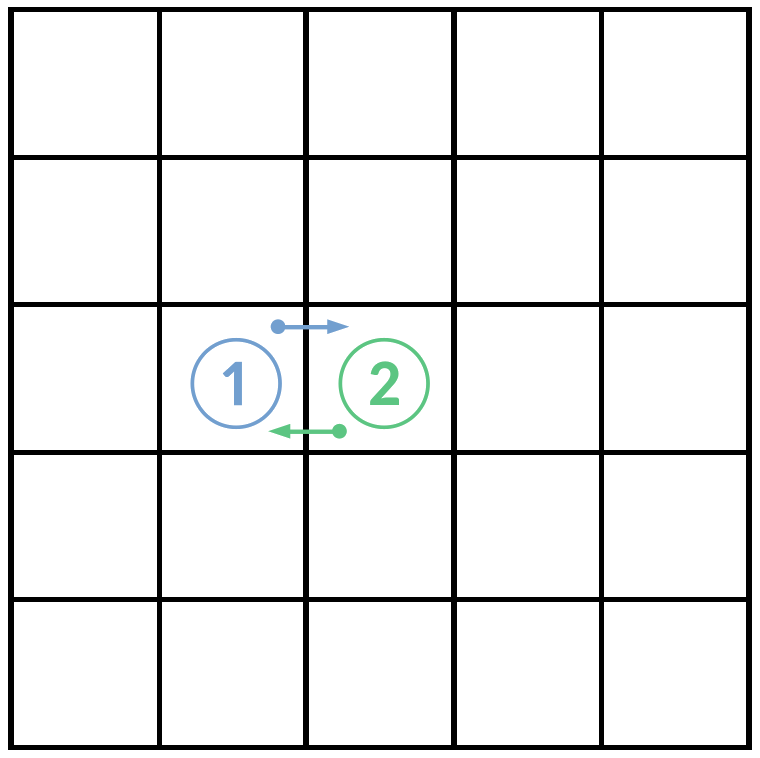
\includegraphics[width=200px]{images/switch.png}
\end{figure}

Dans cette situation, l'agent \circled{1} souhaite se rendre sur la case située à droite de l'agent \circled{2} qui lui veut aller sur la case occupée par l'agent \circled{1}. Les deux agents s'envoyant des messages contradictoire, l'un va comprendre qu'il doit effectuer un mouvement orthogonal par rapport à l'autre agent afin de le laisser passer pour ensuite rejoindre sa place.


\subsection{Le cas à trois agents}

Dans cette situation, on peut faire face à un nouveau cas pathologique.

\begin{figure}[h]
	\centering
	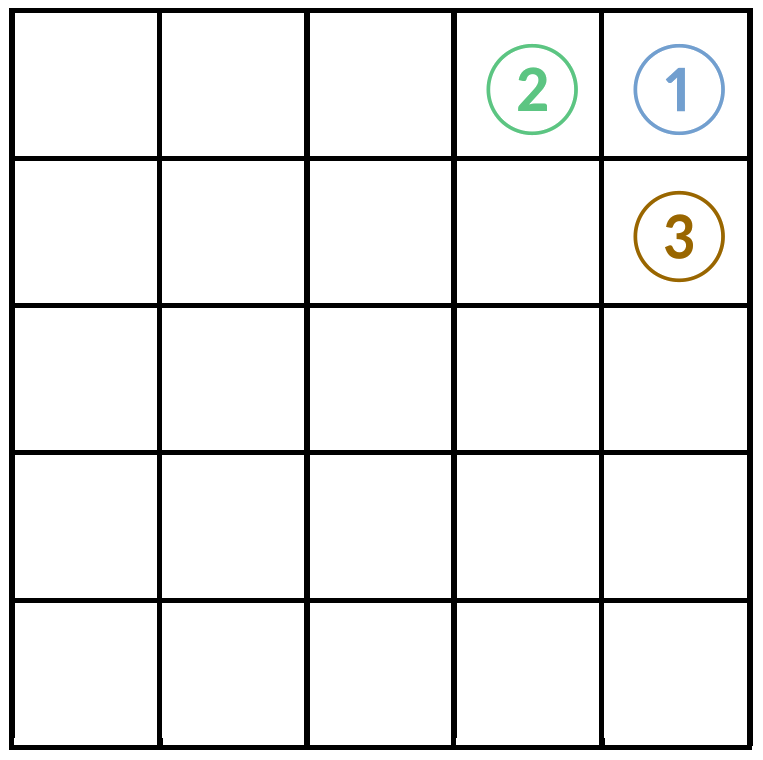
\includegraphics[width=200px]{images/3_agents.png}
\end{figure}

L’agent \circled{1} n'est pas sur sa case d'objectif et est ici \og{} enfermé \fg{} : il n'a aucun mouvement possible, c'est pourquoi il envoie un message à tous ses voisins pour leur demander de bouger.

\subsection{Le cas à quatre agents}

\begin{figure}[h]
	\centering
	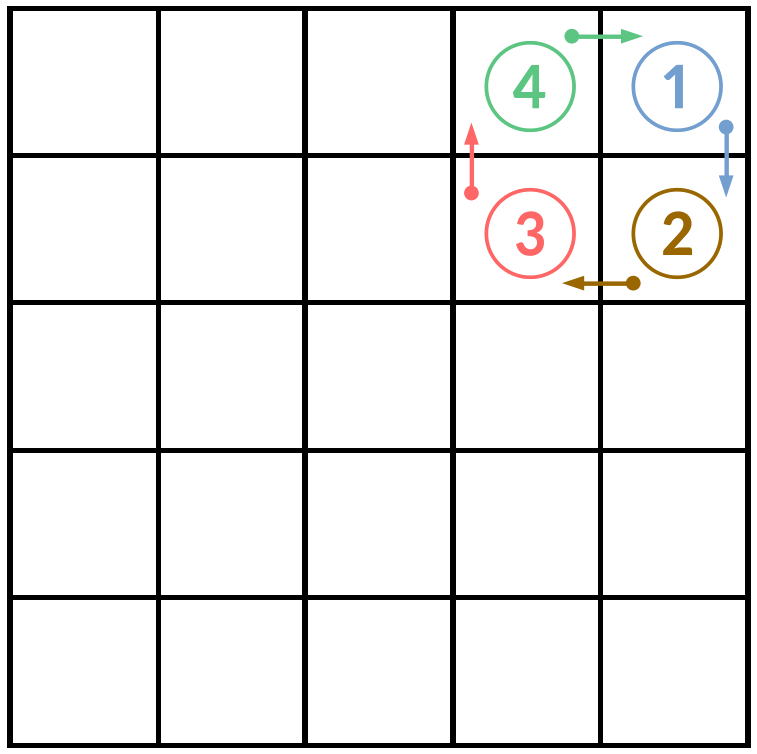
\includegraphics[width=200px]{images/4_agents.png}
\end{figure}

Nous faisons désormais face à un cycle où chaque agent $i$ souhaite aller sur la case occupée par l'agent $i + 1$, qui est en réalité une généralisation du cas évoqué plus haut pour deux agents qui souhaite aller dans des directions opposées en se \og{} croisant \fg{}. La résolution se fait de la même manière : un des agents va prendre la décision d'effectuer un mouvement orthogonal pour \og{} sortir du carré \fg{} et permettre au système de se résoudre.

\subsection{Le cas à cinq agents}

Le dernier cas pathologique présenté ci-dessous se déroule sur une grille avec 5 agents, mais ressemble quelque peu au cas pathologique avec deux agents. Les agents \circled{2}, \circled{3} et \circled{5} sont à leur case d'objectif et ne souhaitent donc pas bouger. Les agents \circled{1} et \circled{4} doivent \og{} intervertir \fg{} leurs places mais aucun ne peut effectuer un mouvement orthogonal, et se contentent de \og{} monter \fg{} et \og{} descendre \fg{}. Au bout d'un certain temps, voyant que rien ne progresse, un des agents va alors effectuer un nombre de mouvements aléatoires défini par la constante \texttt{RANDOM\_MOVE}. Cela va permettre de suffisamment l'éloigner de la situation bloquée pour qu'il trouve un autre chemin dans la grille.

\begin{figure}[h]
	\centering
	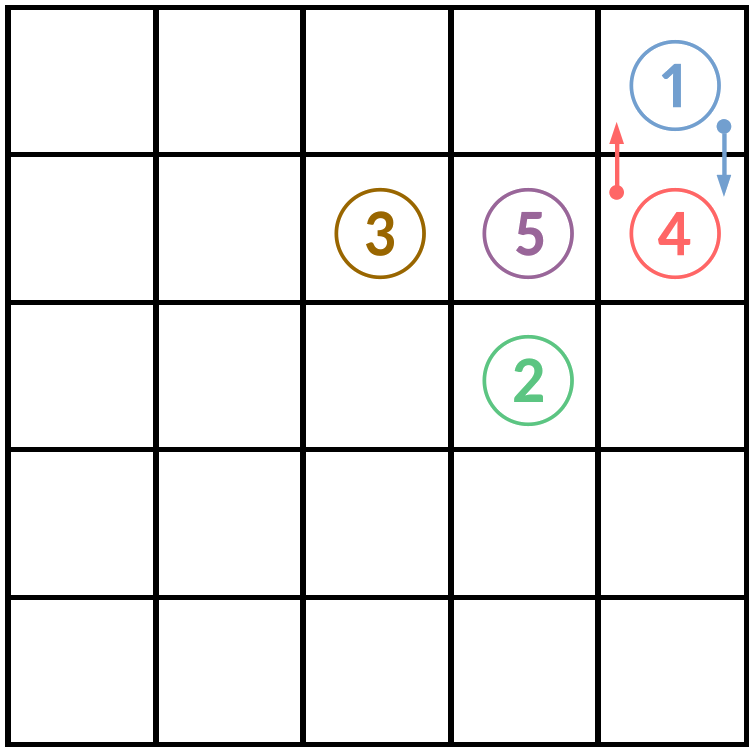
\includegraphics[width=200px]{images/5_agents.png}
\end{figure}

\section{Conclusion}

\end{document}
